% Telos shared preamble.
%
% Every Telos publication is designed to be printed on a home laser printer,
% one sheet at a time, and carried into a boat or a garage. Two constraints
% follow from that and govern everything below:
%
%   1. Pure monochrome. No value is ever a hue. Emphasis is carried by rule
%      weight, fill, and type, never by color, so a grayscale or black-only
%      printer loses nothing.
%   2. Card density. A "one-pager" is a hard contract: the leaf must fit on a
%      single side of US Letter. The layout is therefore tight by default and
%      the environments below are sized to leave room for a plate.

\documentclass[10pt,letterpaper]{article}

\usepackage[margin=0.55in,includefoot,footskip=0.24in]{geometry}
\usepackage[T1]{fontenc}
\usepackage[utf8]{inputenc}
\usepackage{lmodern}
\usepackage{microtype}
\usepackage{array}
\usepackage{booktabs}
\usepackage{longtable}
\usepackage{tabularx}
\usepackage{enumitem}
\usepackage{needspace}
\usepackage{multicol}
\usepackage{ragged2e}
\usepackage{graphicx}
\usepackage{wrapfig}
\usepackage{xcolor}
\usepackage{fancyhdr}
\usepackage{titlesec}
\usepackage{hyperref}
\usepackage[most]{tcolorbox}
\usepackage{tikz}
\usetikzlibrary{arrows.meta,calc,positioning,shapes.geometric,decorations.pathmorphing,patterns,fadings}

% Semantic names are kept so a document reads intelligibly, but every value is
% black, white, or a neutral gray that survives a black-only print driver.
\definecolor{telosink}{gray}{0}
\definecolor{telospaper}{gray}{1}
\definecolor{telosrule}{gray}{0.35}
\definecolor{telosfill}{gray}{0.90}
\definecolor{telosdeep}{gray}{0.72}
\definecolor{telosmute}{gray}{0.45}

\hypersetup{hidelinks,pdfborder={0 0 0}}

% Keep an unchanged source byte-reproducible across rebuilds: no build-clock
% creation date and no random trailer ID.
\pdfinfoomitdate=1
\pdftrailerid{}

\setlength{\parindent}{0pt}
\setlength{\parskip}{0.42em}
\setlength{\tabcolsep}{4pt}
\setlength{\columnsep}{1.1em}
\renewcommand{\arraystretch}{1.18}
\setlist[itemize]{leftmargin=1.15em,itemsep=0.12em,topsep=0.2em,parsep=0pt}
\setlist[enumerate]{leftmargin=1.5em,itemsep=0.18em,topsep=0.2em,parsep=0pt}
\setlist[description]{leftmargin=0pt,itemsep=0.16em,topsep=0.2em,parsep=0pt,
  font=\normalfont\bfseries}

% ---------------------------------------------------------------------------
% Document identity. Each leaf declares these before \begin{document} so the
% running head, the colophon, and the PDF metadata all agree.
% ---------------------------------------------------------------------------
\newcommand{\TelosProject}{Telos}
\newcommand{\TelosDocTitle}{}
\newcommand{\TelosDocSubtitle}{}
\newcommand{\TelosRevision}{}

\newcommand{\telosmeta}[4]{%
  \renewcommand{\TelosProject}{#1}%
  \renewcommand{\TelosDocTitle}{#2}%
  \renewcommand{\TelosDocSubtitle}{#3}%
  \renewcommand{\TelosRevision}{#4}%
  \hypersetup{pdftitle={#2},pdfsubject={#3; version #4},
    pdfkeywords={Telos, version #4},pdfauthor={Telos}}%
}

\pagestyle{fancy}
\fancyhf{}
\renewcommand{\headrulewidth}{0pt}
\renewcommand{\footrulewidth}{0.4pt}
\fancyfoot[L]{\footnotesize\textsc{\TelosProject}}
\fancyfoot[C]{\footnotesize\TelosDocTitle}
\fancyfoot[R]{\footnotesize\thepage}

% The first page of a one-pager carries the masthead instead of a running foot,
% so its footer is the compact provenance line.
\fancypagestyle{telosfirst}{%
  \fancyhf{}%
  \renewcommand{\headrulewidth}{0pt}%
  \renewcommand{\footrulewidth}{0.4pt}%
  \fancyfoot[L]{\footnotesize\textsc{\TelosProject}}%
  \fancyfoot[C]{\footnotesize\TelosRevision}%
  \fancyfoot[R]{\footnotesize\thepage}%
}

% ---------------------------------------------------------------------------
% Masthead. A heavy rule, the title, a light subtitle, a thin rule. The
% optional argument is a right-aligned tag (a species' scientific name, a
% lesson number) that sits on the title's baseline.
% ---------------------------------------------------------------------------
\newcommand{\telosmasthead}[1][]{%
  \thispagestyle{telosfirst}%
  \begingroup
  \setlength{\parskip}{0pt}%
  \noindent\rule{\linewidth}{1.6pt}\par
  \vspace{0.30em}
  \noindent
  \begin{minipage}[b]{0.66\linewidth}
    \raggedright{\LARGE\bfseries\TelosDocTitle}
  \end{minipage}%
  \hfill
  \begin{minipage}[b]{0.32\linewidth}
    \raggedleft{\small\itshape #1}
  \end{minipage}\par
  \vspace{0.18em}
  \noindent{\small\TelosDocSubtitle}\par
  \vspace{0.28em}
  \noindent\rule{\linewidth}{0.4pt}\par
  \endgroup
  \vspace{0.35em}
}

% ---------------------------------------------------------------------------
% Headings. Compact, small-caps, rule-anchored — a card has no room for the
% article class's default vertical air.
% ---------------------------------------------------------------------------
\titleformat{\section}{\normalfont\large\bfseries}{}{0pt}{}[\vspace{-0.55em}\rule{\linewidth}{0.4pt}]
\titlespacing*{\section}{0pt}{0.85em}{0.35em}
\titleformat{\subsection}{\normalfont\normalsize\bfseries}{}{0pt}{}
\titlespacing*{\subsection}{0pt}{0.6em}{0.2em}
\titleformat{\subsubsection}{\normalfont\small\bfseries\scshape}{}{0pt}{}
\titlespacing*{\subsubsection}{0pt}{0.45em}{0.12em}

% A short run-in heading for card interiors that must not consume a full line.
\newcommand{\telosrubric}[1]{\textbf{#1}\enspace}

% Cross-reference helper. Every Telos project is a set of loose printed sheets,
% so a reference names the sheet rather than a page number.
\newcommand{\sheetref}[1]{\textit{see the \textbf{#1} sheet}}

% Which decision, ADR or sheet governs the paragraph you are reading. A reader
% who disagrees with an instruction should be able to find the reasoning behind
% it rather than having to take it on trust.
\newcommand{\governedby}[1]{{\footnotesize\textsc{governed by #1}}}

% ---------------------------------------------------------------------------
% Quantities. siunitx is not in this TeX Live split, and the guides need only a
% fixed thin space and upright units, so define that directly rather than take
% a package dependency the documented install would not satisfy.
%   \qty{9}{kV}  ->  9 kV        \unitof{kV}  ->  kV
% ---------------------------------------------------------------------------
\newcommand{\unitof}[1]{\ensuremath{\mathrm{#1}}}
\newcommand{\qty}[2]{#1\,\unitof{#2}}
\newcommand{\numrange}[2]{#1\,--\,#2}
\newcommand{\qtyrange}[3]{#1\,--\,#2\,\unitof{#3}}
% Inches and feet appear constantly in the fishing guide; keep one spelling.
\newcommand{\inch}[1]{#1\,in}
\newcommand{\feet}[1]{#1\,ft}

% ---------------------------------------------------------------------------
% Cards and boxes.
% ---------------------------------------------------------------------------

% Titled card with a hairline frame. The default card for facts a reader looks
% up rather than reads through.
\newtcolorbox{teloscard}[1]{
  enhanced, breakable,
  colback=telospaper, colframe=telosink, colbacktitle=telospaper,
  coltitle=telosink,
  boxrule=0.5pt, sharp corners,
  left=6pt, right=6pt, top=4pt, bottom=4pt,
  toptitle=3pt, bottomtitle=3pt, titlerule=0.4pt,
  before skip=6pt, after skip=6pt,
  title={#1}, fonttitle=\small\bfseries
}

% Untitled left-ruled block: hierarchy without a redundant label.
\newtcolorbox{telosframe}{
  enhanced, breakable,
  colback=telospaper, frame hidden, boxrule=0pt, sharp corners,
  borderline west={1.3pt}{0pt}{telosink},
  left=8pt, right=2pt, top=3pt, bottom=3pt,
  before skip=6pt, after skip=6pt
}

% Filled emphasis panel — the "read this first" block. The 10% fill stays
% legible under a cheap laser toner curve and still reads as distinct.
\newtcolorbox{telospanel}[1]{
  enhanced, breakable,
  colback=telosfill, colframe=telosink, colbacktitle=telosfill,
  coltitle=telosink,
  boxrule=0.5pt, sharp corners,
  left=6pt, right=6pt, top=4pt, bottom=4pt,
  toptitle=3pt, bottomtitle=3pt, titlerule=0.4pt,
  before skip=6pt, after skip=6pt,
  title={#1}, fonttitle=\small\bfseries
}

% Hazard block. Deliberately the heaviest object on any page: a 1.4pt frame
% plus a solid title bar. Nothing else in Telos is allowed to look like this,
% so a reader skimming a lesson cannot mistake it for ordinary emphasis.
\newtcolorbox{teloshazard}[1]{
  enhanced, breakable,
  colback=telospaper, colframe=telosink,
  colbacktitle=telosink, coltitle=telospaper,
  boxrule=1.4pt, sharp corners,
  left=6pt, right=6pt, top=5pt, bottom=5pt,
  toptitle=3pt, bottomtitle=3pt,
  before skip=8pt, after skip=8pt,
  title={\MakeUppercase{#1}}, fonttitle=\small\bfseries
}

% A stop-and-check gate. Used before anything destructive, and before anything
% that would be expensive to discover later. Shared by every project that has
% a procedure someone could get hurt following carelessly.
\newtcolorbox{gate}[1]{
  enhanced, breakable,
  colback=telospaper, colframe=telosink,
  boxrule=1.0pt, sharp corners,
  left=6pt, right=6pt, top=4pt, bottom=4pt,
  toptitle=3pt, bottomtitle=3pt, titlerule=0.4pt,
  before skip=7pt, after skip=7pt,
  colbacktitle=telospaper, coltitle=telosink,
  title={\MakeUppercase{#1}}, fonttitle=\small\bfseries
}

% ---------------------------------------------------------------------------
% Rating dots. A five-step scale that prints identically in black-only: filled
% versus open circles, never a shaded bar.
% ---------------------------------------------------------------------------
\newcommand{\telosdot}{\tikz[baseline=-0.42ex]\fill[telosink] (0,0) circle (0.28ex);}
\newcommand{\telosopendot}{\tikz[baseline=-0.42ex]\draw[telosink,line width=0.28pt] (0,0) circle (0.28ex);}
\makeatletter
\newcounter{telos@rate}
\newcommand{\telosrating}[1]{%
  \begingroup
  \setcounter{telos@rate}{0}%
  \@whilenum\value{telos@rate}<#1\do{\telosdot\kern0.22em\stepcounter{telos@rate}}%
  \@whilenum\value{telos@rate}<5\do{\telosopendot\kern0.22em\stepcounter{telos@rate}}%
  \endgroup
}
\makeatother

% ---------------------------------------------------------------------------
% Tables.
%
% tabularx reads its body by scanning for a literal \end{tabularx}, so it can
% never be wrapped in a \newenvironment. Documents therefore open tabularx and
% longtable directly and take their house style from these column types and the
% booktabs rules. The one exception is the fact strip below, which is built on
% plain tabular precisely so it *can* be an environment.
% ---------------------------------------------------------------------------
\newcolumntype{L}{>{\raggedright\arraybackslash}X}
\newcolumntype{R}{>{\raggedleft\arraybackslash}X}
\newcolumntype{C}{>{\centering\arraybackslash}X}
\newcolumntype{B}{>{\bfseries\raggedright\arraybackslash}X}
\newcolumntype{N}{>{\raggedright\arraybackslash}p{0.16\linewidth}}

% Key/value fact strip. Two flush columns of short lookups; the label column is
% a fixed fraction so a stack of cards aligns across the whole guide.
\newenvironment{telosfacts}[1][0.24]
  {\begingroup\small
   \setlength{\parskip}{0pt}%
   \renewcommand{\arraystretch}{1.25}%
   \begin{tabular}{@{}>{\bfseries\raggedright\arraybackslash}p{\dimexpr#1\linewidth\relax}@{\hspace{0.7em}}>{\raggedright\arraybackslash}p{\dimexpr\linewidth-#1\linewidth-0.7em\relax}@{}}}
  {\end{tabular}\par\endgroup}
\newcommand{\telosfact}[2]{#1 & #2\\}

% ---------------------------------------------------------------------------
% Seasonal / diurnal activity bar.
%
% \telosseasonbar{4,3,2,1,1,2,3,3,4,5,4,3} draws a twelve-cell month strip
% where each value 0-5 is a fill height. Height, not gray value, carries the
% signal, so it is exact under any toner curve; the cell is outlined either way
% so an empty month is still visibly a month.
% ---------------------------------------------------------------------------
\newcommand{\telosseasonlabels}{J,F,M,A,M,J,J,A,S,O,N,D}
\newcommand{\telosseasonbar}[1]{%
  \begingroup
  \begin{tikzpicture}[x=1.25em,y=2.1ex,baseline=0pt]
    \foreach \v [count=\i from 0] in {#1} {
      \draw[telosrule,line width=0.3pt] (\i,0) rectangle (\i+0.86,5);
      \ifnum\v>0
        \fill[telosink] (\i,0) rectangle (\i+0.86,\v);
      \fi
    }
    \foreach \m [count=\i from 0] in \telosseasonlabels {
      \node[font=\tiny,anchor=north,inner sep=1.2pt] at (\i+0.43,-0.1) {\m};
    }
  \end{tikzpicture}%
  \endgroup
}

% Four-cell day-part strip: dawn, midday, dusk, night.
\newcommand{\telosdaylabels}{Dawn,Mid,Dusk,Night}
\newcommand{\telosdaybar}[1]{%
  \begingroup
  \begin{tikzpicture}[x=2.9em,y=2.1ex,baseline=0pt]
    \foreach \v [count=\i from 0] in {#1} {
      \draw[telosrule,line width=0.3pt] (\i,0) rectangle (\i+0.92,5);
      \ifnum\v>0
        \fill[telosink] (\i,0) rectangle (\i+0.92,\v);
      \fi
    }
    \foreach \m [count=\i from 0] in \telosdaylabels {
      \node[font=\tiny,anchor=north,inner sep=1.2pt] at (\i+0.46,-0.1) {\m};
    }
  \end{tikzpicture}%
  \endgroup
}

% A bar needs vertical room for its labels when it sits in a fact strip.
\newcommand{\telosbarrow}[1]{\rule{0pt}{4.2ex}#1\rule[-1.6ex]{0pt}{1.6ex}}

% ---------------------------------------------------------------------------
% Plates. A species or apparatus illustration with a caption rule beneath it.
% \telosplate{width fraction}{file}{caption}
% ---------------------------------------------------------------------------
\newcommand{\telosplate}[3]{%
  \begingroup
  \centering
  \includegraphics[width=#1\linewidth]{#2}\par
  \vspace{0.15em}
  \begin{minipage}{#1\linewidth}
    \rule{\linewidth}{0.4pt}\par
    \vspace{0.1em}
    {\footnotesize #3\par}
  \end{minipage}\par
  \endgroup
  \vspace{0.3em}
}

% TikZ drawing conventions shared by every rig, knot, and circuit diagram.
\tikzset{
  telos line/.style={draw=telosink,line width=0.7pt},
  telos hair/.style={draw=telosink,line width=0.35pt},
  telos heavy/.style={draw=telosink,line width=1.2pt},
  telos node/.style={draw=telosink,fill=telospaper,align=center,inner sep=4pt,font=\small},
  telos emphasis/.style={draw=telosink,line width=1.2pt,fill=telospaper,align=center,
    inner sep=4pt,font=\small\bfseries},
  telos label/.style={font=\scriptsize,inner sep=1.5pt},
  telos arrow/.style={-{Stealth[length=1.8mm]},draw=telosink,line width=0.6pt},
  telos dim/.style={|<->|,draw=telosink,line width=0.35pt},
  telos water/.style={draw=telosrule,line width=0.4pt,decorate,
    decoration={snake,amplitude=0.4mm,segment length=3mm}},
}

% ---------------------------------------------------------------------------
% Lesson furniture
% ---------------------------------------------------------------------------

% \lessonhead{number}{time}{who does what}
\newcommand{\lessonhead}[3]{%
  \par\noindent
  \begin{minipage}{\linewidth}
    \rule{\linewidth}{0.4pt}\par
    \vspace{0.3em}
    {\small\textbf{Lesson #1}\quad$\cdot$\quad #2\quad$\cdot$\quad #3\par}
    \vspace{0.25em}
    \rule{\linewidth}{0.4pt}
  \end{minipage}\par
  \vspace{0.5em}}

% The materials list. Two columns of short lines; a lesson that needs a long
% shopping list is a lesson that has not been thought through.
\newenvironment{materials}
  {\begin{telospanel}{What you need}\begin{multicols}{2}
   \begin{itemize}[leftmargin=1em,itemsep=0.05em,topsep=0pt]}
  {\end{itemize}\end{multicols}\end{telospanel}}

% The four rubrics every lesson carries, in the same order every time:
% what you are about to see, what to do, what it means, and what to ask.
\newcommand{\lessonsection}[1]{\section*{#1}\vspace{-0.35em}\rule{\linewidth}{0.4pt}\vspace{0.2em}}

% A prediction box. The point of the curriculum is that they commit to an
% answer before the demonstration, not after.
\newtcolorbox{predict}{
  enhanced, breakable,
  colback=telospaper, colframe=telosink,
  boxrule=0.5pt, sharp corners,
  left=6pt, right=6pt, top=4pt, bottom=4pt,
  before skip=6pt, after skip=6pt,
  borderline west={2.2pt}{0pt}{telosink},
  title={\small\bfseries Predict first}, fonttitle=\small\bfseries,
  colbacktitle=telospaper, coltitle=telosink,
  toptitle=3pt, bottomtitle=3pt, titlerule=0.4pt,
}

% ---------------------------------------------------------------------------
% Colophon. Rendered once, at the end of the last page, in the recovered footer
% area so it never creates a page of its own.
% ---------------------------------------------------------------------------
\newif\ifTelosColophonRendered
\newcommand{\TelosColophonExtra}{}
\newcommand{\TelosColophon}{%
  \ifTelosColophonRendered\else
  \global\TelosColophonRenderedtrue
  \par
  \enlargethispage{0.5in}%
  \vspace{0.3em}%
  \begingroup
  \setlength{\parskip}{0pt}%
  \begin{minipage}{\linewidth}
  \rule{\linewidth}{0.35pt}\par
  \vspace{0.3em}%
  \fontsize{7}{8.2}\selectfont
  \textbf{Telos.} \TelosProject{} — \TelosDocTitle. Revised \TelosRevision.
  \TelosColophonExtra{}
  Project-created text and diagrams are licensed \href{https://creativecommons.org/licenses/by/4.0/}{CC BY 4.0}.
  Incorporated public-domain artwork remains public domain and is credited on
  the plate it appears with. See \texttt{LICENSE} and \texttt{CREDITS.md} in the
  source. Nothing here is professional advice; verify current regulations and
  follow the stated safety procedure.
  \end{minipage}
  \endgroup
  \fi
}
\AtEndDocument{\TelosColophon}

% Shared macros for the homelab project.
%
% This project's documents are read in two very different situations: at a desk
% while designing, and standing in front of a broken machine at eleven at night
% with no network. The second case is the one that sets the style. Commands are
% set apart so they can be found by eye, every dangerous step has a visible
% verification after it, and nothing depends on being able to reach a web page.

% ---------------------------------------------------------------------------
% Decision-record entries, used by the generated digest.
% ---------------------------------------------------------------------------
\newcommand{\adrentry}[4]{%
  \par\vspace{0.7em}
  \needspace{4\baselineskip}%
  \noindent
  \begin{minipage}{\linewidth}
    \rule{\linewidth}{0.6pt}\par
    \vspace{0.25em}
    {\small\textbf{ADR #1}\quad #2\par}
    \vspace{0.1em}
    {\fontsize{7}{8.2}\selectfont\textsc{#3}\quad$\cdot$\quad #4\par}
    \vspace{0.2em}
    \rule{\linewidth}{0.3pt}
  \end{minipage}\par
  \vspace{0.3em}}

% ---------------------------------------------------------------------------
% Procedures.
%
% A rebuild manual is a sequence of commands and the observable evidence that
% each one worked. These environments keep that pairing structural rather than
% a matter of the author remembering.
% ---------------------------------------------------------------------------

% A block of shell to type. Deliberately not a listing package: plain verbatim
% in a ruled box prints identically everywhere and has no font dependency.
\newenvironment{shellblock}
  {\par\vspace{0.25em}\noindent
   \begin{minipage}{\linewidth}
   \rule{\linewidth}{0.3pt}\par\vspace{0.15em}
   \begingroup\footnotesize\ttfamily\obeylines\obeyspaces\parindent=0pt\parskip=0pt}
  {\endgroup\par\vspace{0.15em}\rule{\linewidth}{0.3pt}\end{minipage}\par\vspace{0.25em}}

% What you should see if the previous step worked. A step without one of these
% is a step you cannot verify, and in a rebuild manual that is a defect.
\newcommand{\expectthis}[1]{%
  \par\vspace{0.1em}
  \noindent\begin{minipage}{\linewidth}
  \hspace*{0.6em}\begin{minipage}{\dimexpr\linewidth-0.6em\relax}
  {\footnotesize\textbf{Expect:} #1\par}
  \end{minipage}\end{minipage}\par\vspace{0.3em}}

% \begin{gate} now lives in common/preamble.tex, shared with the other
% projects that document procedures.

% \governedby now lives in common/preamble.tex.

% An instance value that comes from the private overlay. In the published
% documents these render as visible placeholders, which is deliberate: a
% published manual must be complete and obviously generic, never look like it
% is describing somebody's actual network.
\newcommand{\instancevalue}[2]{\texttt{\textlangle #1\textrangle}%
  \footnote{Instance value. Supplied from \texttt{homelab/instance/} at build
  time; #2.}}
\newcommand{\placeholder}[1]{\texttt{\textlangle #1\textrangle}}

% ---------------------------------------------------------------------------
% Role and boundary diagrams.
% ---------------------------------------------------------------------------
\tikzset{
  role/.style={draw=telosink,line width=0.9pt,fill=telospaper,align=center,
    inner sep=5pt,font=\small,minimum width=2.6cm},
  roleoff/.style={draw=telosmute,line width=0.5pt,dash pattern=on 2.5pt off 1.8pt,
    fill=telospaper,align=center,inner sep=5pt,font=\small,minimum width=2.6cm},
  boundary/.style={draw=telosmute,line width=0.5pt,dash pattern=on 3pt off 2pt,
    rounded corners=3pt},
  flow/.style={-{Stealth[length=2mm]},draw=telosink,line width=0.7pt},
  hlabel/.style={font=\fontsize{6.4}{7.4}\selectfont},
}


\telosmeta{Homelab}{Network Design}
  {A small, legible network that can grow without becoming vague}{20260727.001}

\begin{document}
\telosmasthead[High-level design]

This design turns one ordinary UniFi LAN into several small trust zones without
renumbering everything at once.  It favours memorable names and addresses, but
keeps the binary subnet boundaries that routers require.  Every change has a
proof step and a retreat path.  Private instance values---people, device
identifiers, keys and exact assignments---belong in the private instance
repository, not in this publication.

\section{Rules that do not move}
\begin{telosfacts}[0.22]
\telosfact{One site root}{The first site uses a private \texttt{10.1} root.  This is an allocation convention, not one enormous scannable subnet.}
\telosfact{Small active ranges}{Each zone receives the smallest power-of-two subnet with between roughly two and ten times its expected population.  Growth is deliberate; scans target one CIDR at a time.}
\telosfact{Human first}{Gateways normally end in \texttt{.1}; durable services take the next simple addresses; people use DNS names rather than memorising numbers.}
\telosfact{One DHCP authority}{UniFi assigns addresses.  A boot server supplies files, not competing leases.  PXE information is attached only to the provisioning network.}
\telosfact{Deny between zones}{A new zone may reach nothing until its required flows are named.  Internet access, DNS, identity, storage and administration are separate permissions.}
\telosfact{Public pattern, private instance}{This document contains roles and placeholders.  The private inventory contains usernames, hostnames, serials, MAC addresses, reservations, share names and actual CIDRs.  Secrets remain encrypted even there.}
\end{telosfacts}

\section{Addressing model}
Subnetting is binary even when the visible plan uses decimal-friendly labels.
A ten-address subnet is not a valid routing boundary; a \texttt{/28} provides
14 usable addresses.  The operator sees the gateway at the first usable
address and a short, documented range.  Unused addresses are not advertised as
another network.

\begin{tabularx}{\linewidth}{@{}p{.14\linewidth}p{.15\linewidth}p{.18\linewidth}L@{}}
\toprule
\textbf{Expected now} & \textbf{Initial CIDR} & \textbf{Usable addresses} & \textbf{Expansion decision}\\
\midrule
1--3 & \texttt{/29} & 6 & Use only for genuinely fixed, tiny roles; reserve an adjacent block.\\
4--7 & \texttt{/28} & 14 & Default for a small appliance class.\\
8--15 & \texttt{/27} & 30 & Default for workstations or a growing device class.\\
16--30 & \texttt{/26} & 62 & Use only when the inventory already justifies it.\\
\bottomrule
\end{tabularx}

\begin{telospanel}{Capacity rule}
Review a zone at 70 percent occupancy.  Expansion is a planned subnet change,
not a reason to begin with a \texttt{/16} or scan an entire private address block.
Reserve nearby address space in the plan, but create only the network in use.
\end{telospanel}

\subsection*{Zone register}
Zone numbers should be memorable decimal labels, commonly in tens.  They do
not have to equal an IP octet or encode security policy.  The private instance
file binds each placeholder to an exact VLAN and CIDR.

\begin{tabularx}{\linewidth}{@{}p{.18\linewidth}p{.17\linewidth}p{.20\linewidth}L@{}}
\toprule
\textbf{Zone role} & \textbf{VLAN placeholder} & \textbf{Initial size} & \textbf{Purpose}\\
\midrule
Management & \texttt{VLAN\_MGMT} & \texttt{/28} & UniFi consoles, switches and access points; administrator devices only.\\
Identity and boot & \texttt{VLAN\_CORE} & \texttt{/28} & AD DNS, Kerberos, directory and boot publication services.\\
Storage & \texttt{VLAN\_STORAGE} & \texttt{/28} & Primary and backup storage appliances; no ordinary client membership.\\
Provisioning & \texttt{VLAN\_BUILD} & \texttt{/28} & Wired, short-lived workstation installation boundary.\\
Managed workstations & \texttt{VLAN\_WORKSTATION} & \texttt{/27} & Installed Windows and Arch clients.\\
Trusted personal & \texttt{VLAN\_TRUSTED} & \texttt{/27} & Personal clients not yet under workstation management.\\
Printers and media & \texttt{VLAN\_DEVICE} & \texttt{/28} & Devices needing narrow, explicit inbound access.\\
IoT & \texttt{VLAN\_IOT} & \texttt{/27} & Untrusted household appliances; no lateral access.\\
Cameras & \texttt{VLAN\_CAMERA} & \texttt{/28} & Cameras and recorder flows only.\\
Guests & \texttt{VLAN\_GUEST} & \texttt{/27} & Internet only, client isolation enabled.\\
\bottomrule
\end{tabularx}

\subsection*{Host-address convention}
Within a zone, \texttt{.1} is the gateway.  Prefer \texttt{.2} through
\texttt{.9} for durable infrastructure, keeping fixed addresses outside the
dynamic pool.  Use DHCP reservations by DNS name for ordinary devices.
A trailing zero appears only in unavoidable CIDR notation, never as a host
address someone must type.  For example, a zone labelled 40 may occupy only
\placeholder{zone-cidr}; the label does not justify routing or scanning its
whole parent allocation.

\section{Traffic contract}
\begin{center}
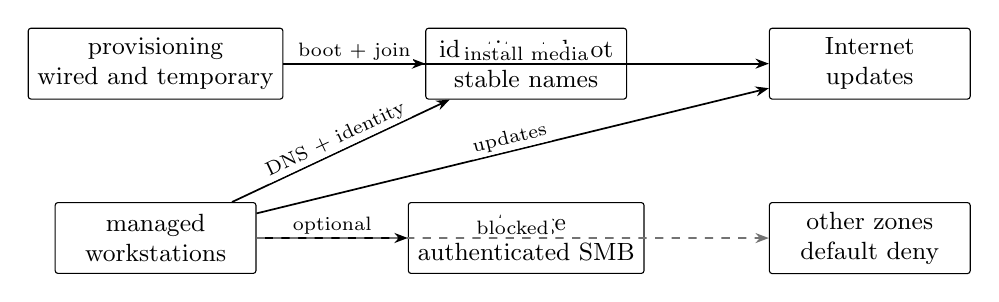
\begin{tikzpicture}[
  box/.style={draw=telosink,rounded corners=1pt,fill=telospaper,
    minimum width=2.55cm,minimum height=.9cm,align=center,font=\small},
  flow/.style={-{Stealth[length=1.7mm]},line width=.62pt},
  denied/.style={flow,dashed,draw=telosmute},
  note/.style={font=\scriptsize,align=center,fill=telospaper,inner sep=1pt}]
\node[box] (build) {provisioning\\wired and temporary};
\node[box,right=18mm of build] (core) {identity + boot\\stable names};
\node[box,right=18mm of core] (wan) {Internet\\updates};
\node[box,below=13mm of build] (ws) {managed\\workstations};
\node[box,below=13mm of core] (store) {storage\\authenticated SMB};
\node[box,below=13mm of wan] (other) {other zones\\default deny};
\draw[flow] (build)--node[note,above]{boot + join}(core);
\draw[flow] (build)--node[note,above]{install media}(wan);
\draw[flow] (ws)--node[note,above,sloped]{DNS + identity}(core);
\draw[flow] (ws)--node[note,above]{optional}(store);
\draw[flow] (ws)--node[note,above,sloped]{updates}(wan);
\draw[denied] (ws)--node[note,above]{blocked}(other);
\end{tikzpicture}
\end{center}

The matrix below is the source of truth.  ``Required'' still means the rule is
limited by source, destination and service; it never means \emph{allow any}.

\begin{tabularx}{\linewidth}{@{}p{.19\linewidth}p{.22\linewidth}p{.20\linewidth}L@{}}
\toprule
\textbf{Source} & \textbf{Destination} & \textbf{Policy} & \textbf{Proof}\\
\midrule
Managed workstation & AD DNS and identity aliases & Required named services & DNS SRV query, clock check, Kerberos ticket and directory login.\\
Managed workstation & Storage alias & Optional authenticated SMB & Mapping succeeds when present; login still succeeds when storage is blocked.\\
Managed workstation & Internet & Required update traffic & Windows and Arch metadata fetch through ordinary DNS; no access to management.\\
Provisioning client & Boot alias and install sources & Required during a build & DHCP lease, boot filename, iPXE fetch and artifact checksum recorded.\\
Administrator device & Management zone & Required from explicit sources & Console opens from the allowed source and fails from a workstation.\\
Guest, IoT, camera & Private zones & Denied unless a narrow exception exists & Attempted DNS, HTTPS and SMB probes fail; rejection appears in logs.\\
Any client & Peer in same restricted zone & Denied where isolation is promised & Two sacrificial clients cannot exchange test traffic.\\
\bottomrule
\end{tabularx}

\section{UniFi change sequence}
Menu labels can move between Network application releases.  Match the property
named here, not a remembered screen position.  Export a UniFi backup and record
the Network application version before changing anything.

\begin{enumerate}
\item Create the zone's virtual network with its recorded VLAN ID, gateway and
small CIDR.  Keep the UDM as DHCP server.  \textbf{What this does:} creates one
routed broadcast boundary without introducing a second address authority.
\item Set a DHCP pool that excludes the gateway and every fixed reservation.
Set lease duration deliberately.  \textbf{Verify:} a test client receives an
in-range address, the UDM gateway and the intended DNS servers.
\item Assign a sacrificial switch port as an access port for that network.
Do not convert a live host link into a trunk during this proof.
\textbf{Verify:} the port's native network and the client's observed subnet agree.
\item Add required allow rules from the traffic contract, most specific first.
Add the zone-to-zone deny after each required flow has passed.
\textbf{What this does:} makes a missing dependency visible instead of hiding
it behind broad private-network access.
\item Enable logging temporarily on the final deny.  Test one allowed and one
forbidden flow from the sacrificial client.  Remove noisy logging only after
the rule counters and client observations agree.
\item For the provisioning network only, set the DHCP boot server to the stable
boot-service address and the boot filename to the approved x86-64 UEFI iPXE
loader.  \textbf{Verify:} capture the DHCP exchange and confirm that UniFi is
the only DHCPOFFER source.
\item After ordinary DHCP is proven, enable DHCP Guarding on supported UniFi
switches and trust only that network's UDM gateway address.
\textbf{What this does:} rejects rogue DHCP offers and intentionally excludes
Controller ProxyDHCP.  \textbf{Verify:} a normal UDM lease still succeeds; use
an isolated test before generating any deliberate rogue offer.
\end{enumerate}

\begin{telospanel}{Pre-attachment gate}
Before a port or SSID can carry the new zone, confirm all six:
\texttt{[ ]} backup and version recorded;\quad
\texttt{[ ]} CIDR capacity calculated;\quad
\texttt{[ ]} DHCP pool excludes fixed addresses;\quad
\texttt{[ ]} endpoint and service groups exist;\quad
\texttt{[ ]} final deny is logged;\quad
\texttt{[ ]} rollback port profile is recorded.
The operator initials the completed private worksheet; an unchecked item stops
attachment.
\end{telospanel}

\subsection*{Version-sensitive console map}
Use the search box when a label differs.  The object and resulting property are
authoritative; the breadcrumb is only a starting point.

\begin{tabularx}{\linewidth}{@{}p{.20\linewidth}p{.31\linewidth}L@{}}
\toprule
\textbf{Object} & \textbf{Current zone-based releases} & \textbf{Older or alternate label}\\
\midrule
Virtual network & Settings $\rightarrow$ Networks $\rightarrow$ New Virtual Network &
Settings $\rightarrow$ Networks $\rightarrow$ Create New Network\\
Zones & Settings $\rightarrow$ Security $\rightarrow$ Zones &
Implicit LAN, Guest, WAN and Gateway categories\\
Traffic rule & Settings $\rightarrow$ Security $\rightarrow$ Policy Engine &
Settings $\rightarrow$ Firewall \& Security $\rightarrow$ LAN In / Guest In\\
DHCP boot values & Network $\rightarrow$ DHCP Service Management $\rightarrow$ Network Boot &
Network $\rightarrow$ Advanced $\rightarrow$ DHCP Options / TFTP Server\\
Port membership & Devices $\rightarrow$ switch $\rightarrow$ Ports $\rightarrow$ selected port &
Port Manager or a named Switch Port Profile\\
DHCP Guarding & Network or switch security settings &
DHCP Snooping / Guarding under the selected network\\
PPSK & WiFi $\rightarrow$ SSID $\rightarrow$ Security $\rightarrow$ Private Pre-Shared Keys &
WiFi $\rightarrow$ Manual / Advanced security\\
\bottomrule
\end{tabularx}

\begin{telospanel}{Do not translate rule direction by name}
On a zone-based release, express source zone, destination zone and service
directly.  On a legacy release, an inter-VLAN packet is commonly filtered on
the source network's ``In'' chain.  Confirm with a sacrificial packet and the
matched-rule counter; never infer equivalence from a similar-looking label.
\end{telospanel}

\subsection*{Staged zone procedure}
Create policy before attaching a real client.  This avoids the interval in
which a newly routed network inherits broader access than intended.

\begin{enumerate}
\item Freeze a worksheet row: Network application version, backup identifier,
zone name, VLAN, CIDR, gateway, DHCP range, DNS, NTP and expected population.
\item Create address groups for the exact Controller, identity/DNS, storage and
administrator endpoints.  Create service groups from the port matrix below.
\item Create the custom zone, if the installed release supports custom zones.
Add narrow allows for DHCP to the gateway, assigned DNS, time, identity,
updates and any explicitly selected storage service.
\item Add and temporarily log the final inter-zone deny.  Put established and
related return handling where the installed policy model requires it; do not
create a reverse broad allow.
\item Inspect ordering and counters while the zone has no port or SSID.  Save
screenshots or an exported policy list as the pre-attachment record.
\item Create the virtual network and DHCP scope, but attach no production port
or SSID.  Assign one sacrificial access port, renew its lease, and run every
positive and negative probe.
\item Only after evidence matches the plan, attach the intended port profile or
SSID.  Rollback means removing that attachment first; policy objects can remain
disabled for diagnosis.
\end{enumerate}

\section{Service and port contract}
Start with these protocol surfaces, then reduce them from observed service
requirements.  Stateful return traffic is not a separate client-bound allow.
The destination must be an endpoint group, never an entire private root.

\begingroup
\small
\begin{tabularx}{\linewidth}{@{}p{.16\linewidth}p{.20\linewidth}p{.19\linewidth}L@{}}
\toprule
\textbf{Purpose} & \textbf{Source $\rightarrow$ destination} &
\textbf{Transport / port} & \textbf{Verification}\\
\midrule
DHCP & client $\rightarrow$ UDM DHCP & UDP 67--68 &
Capture one discover/offer/request/ack; one server identifier only.\\
DNS & clients $\rightarrow$ AD DNS & TCP/UDP 53 &
Resolve an external name, an AD host and the LDAP/Kerberos SRV records.\\
Time & clients $\rightarrow$ approved NTP & UDP 123 &
Record source, offset and synchronized state.\\
Kerberos & clients $\rightarrow$ domain controllers & TCP/UDP 88; TCP/UDP 464 &
Acquire and inspect a user ticket; test password change separately.\\
Directory & clients $\rightarrow$ domain controllers & TCP/UDP 389; TCP 636 if configured; TCP 3268--3269 when used &
Bind by DNS name and perform the intended directory lookup.\\
AD file/RPC & clients $\rightarrow$ domain controllers & TCP 445, 135; negotiated high TCP RPC range &
Join a disposable client and inspect flows before narrowing the configured RPC range.\\
Boot discovery & build client $\rightarrow$ UDM and boot host & DHCP plus UDP 69 only if the first stage uses TFTP &
Record offered boot server/name and fetch the exact first-stage hash.\\
Boot payload & build client $\rightarrow$ boot publication & TCP 80 or 443 as configured &
Fetch the immutable manifest and verify every checksum.\\
Storage & managed clients $\rightarrow$ named NAS endpoints & TCP 445 &
Authenticate as a test user; then block storage and prove login remains usable.\\
Updates & managed clients $\rightarrow$ Internet & TCP 80/443 via assigned DNS &
Complete a metadata refresh and one signed package verification.\\
Administration & explicit admin sources $\rightarrow$ exact managed endpoints & HTTPS/SSH or vendor ports actually selected &
Connect from an allowed source; repeat from a workstation and observe denial.\\
\bottomrule
\end{tabularx}
\endgroup

\begin{telospanel}{RPC is a design choice}
Windows domain join and management may negotiate dynamic RPC ports.  First
measure a disposable join.  If a smaller range is required, configure the
servers and clients to use that range before narrowing the firewall; simply
blocking the default high range produces intermittent, misleading failures.
\end{telospanel}

\section{Executable proof cycle}
Run the cycle from a named sacrificial client after each network, policy or
service change.  Save commands and timestamps in the private evidence ledger.

\begin{enumerate}
\item \textbf{Link:} record switch port or SSID, client MAC, link speed and
observed VLAN.  A wrong VLAN stops the cycle.
\item \textbf{Lease:} release and renew.  Record address/prefix, gateway, DNS,
lease server and expiry.  Capture DHCP when the authority is ambiguous.
\item \textbf{Name and time:} query external A/AAAA and AD SRV records through
the assigned resolver.  Record the time source and offset.
\item \textbf{Required services:} acquire a Kerberos ticket, perform a directory
lookup, fetch the boot manifest or update metadata, and open only the selected
SMB resource.
\item \textbf{Forbidden neighbours:} probe management, another restricted
client and one unrelated private zone with DNS, TCP connection and application
tests.  Record the exact deny rule or traffic-flow entry.
\item \textbf{Failure injection:} make storage unavailable and prove login
continues; make the boot alias unavailable and prove an installed workstation
still boots locally.
\item \textbf{Restart:} cold-boot the client and repeat the short lease, DNS,
ticket and deny checks.  A cached successful session is not cutover evidence.
\end{enumerate}

\subsection*{Right-sized worked example}
Suppose a role has six devices today and may reach ten before review.  Allocate
one \texttt{/28}: 16 total addresses, 14 usable.  Use the first usable address
as gateway, reserve the next few simple addresses for durable endpoints, and
place the dynamic pool above them.  Record an adjacent unused block for future
growth, but do not create or scan it.  Ten devices consume 71 percent of the
usable addresses, which triggers review.  The private inventory substitutes
the exact CIDR and reservations; the public document never does.

\section{IPv6 phase policy}
Phase one validates IPv4 only.  This is a scope decision, not permission for
unmeasured IPv6.  For every new network, record whether the UDM advertises an
IPv6 prefix, whether clients receive global or unique-local addresses, and
which IPv6 firewall policy applies.  Until an IPv6 traffic contract exists,
disable prefix delegation and router advertisements on these purpose-built
zones where the installed UniFi release permits it, and deny routed IPv6
between trust zones.  Link-local IPv6 remains normal on interfaces.

Before enabling routed IPv6, reproduce the complete IPv4 contract with IPv6
DNS answers, explicit service destinations, positive probes, negative probes,
logging and rollback.  Do not assume an IPv4 deny covers IPv6, and do not call
a network isolated while an untested IPv6 route bypasses its IPv4 policy.

\begin{telospanel}{PXE safety gate}
Do not attach boot options to the ordinary LAN.  A dedicated provisioning
network makes physical attachment part of erase authorization.  Boot options
point to a stable service name or reserved address; a later Controller move
must not require rebuilding workstations.
\end{telospanel}

\begin{telospanel}{AD DNS ordering}
Set clients to the AD DNS address only after that resolver answers both
\texttt{\_ldap.\_tcp.dc.\_msdcs.\placeholder{identity-domain}} and external names. AD clients
must use AD DNS; a resolver with no working forward path makes the Internet
appear broken even when routing is correct.
\end{telospanel}

\section{Managed-workstation Wi-Fi}
The managed SSID is post-install connectivity, not the first firmware PXE
transport.  It maps to the managed-workstation network and has restricted
Internet access.  The household Wi-Fi secret never enters deployment material.

\begin{enumerate}
\item Create the managed-workstation virtual network and prove it on a wired
access port first.  \textbf{Why:} routing and identity failures can then be
separated from radio and credential failures.
\item Create a dedicated SSID mapped to that network.  Use the UniFi-supported
WPA2/PPSK combination when per-device private pre-shared keys are required.
\textbf{Constraint:} PPSK currently excludes WPA3 and 6 GHz; broadcast this
SSID on 2.4 and 5 GHz only.
\item Issue a distinct PPSK per managed workstation and record only its
identifier and assignment in the private inventory.  Store the secret in the
encrypted deployment vault.  \textbf{What this does:} one lost machine can be
revoked without changing every workstation.  A copied PPSK still works from
another device; AD, not the PPSK, establishes user identity.
\item Inject the credential during an authorised build.  The unencrypted
phase-one workstation can still reveal its local credential to a physical
attacker; segmentation limits what that credential can reach but does not make
the disk confidential.
\item Join two test clients.  Verify Internet, AD DNS, Kerberos and optional SMB;
then verify that management, peer clients and other household zones remain
unreachable.
\end{enumerate}

\begin{telospanel}{PPSK capability gate and fallback}
Before designing around PPSK, confirm that the installed access points,
Network release and chosen radio/security mode expose Private Pre-Shared Keys.
PPSK may require WPA2 and may be unavailable with WPA3 or 6\,GHz operation.
If it is unavailable, use a dedicated restricted WPA2 SSID with one deployment
credential as the temporary fallback, rotate it after a lost device, and rely
on AD for user identity.  Prefer 802.1X/RADIUS as the later per-device or
per-user design.  Never silently place managed clients on household Wi-Fi.
\end{telospanel}

\subsection*{When an isolated SSID appears broken}
\begin{tabularx}{\linewidth}{@{}p{.22\linewidth}p{.29\linewidth}L@{}}
\toprule
\textbf{Symptom} & \textbf{Measure first} & \textbf{Likely boundary}\\
\midrule
No address & DHCP exchange and switch/AP network assignment & VLAN not carried to the AP, wrong SSID mapping, or DHCP scope absent.\\
Address but no names & DHCP DNS value; query UDM and AD DNS separately & Firewall omitted DNS or the client received the wrong resolver.\\
Internet but no domain login & Time offset, AD SRV records, Kerberos and LDAP reachability & AD DNS or clock flow missing; broad Internet access is irrelevant.\\
Domain login stalls when NAS is down & Block storage explicitly and time login & Home/share mapping is blocking instead of optional.\\
No peer traffic & Repeat from two clients and inspect isolation setting & Expected on guest-style isolation; disable only if the traffic contract requires peers.\\
Unexpected private access & Test each zone and inspect the matched rule counter & Broad allow precedes the intended deny or the source network is misclassified.\\
\bottomrule
\end{tabularx}

\section{Migration without an outage}
Leave the existing LAN untouched while one new zone is proven.  Start with the
isolated test network, then identity and boot, storage, and managed
workstations.  Move one sacrificial client at a time.  A zone becomes ordinary
only after DHCP, DNS, allowed flows, denied flows, cold reboot and rollback are
all observed.

\begin{tabularx}{\linewidth}{@{}p{.16\linewidth}p{.25\linewidth}L@{}}
\toprule
\textbf{Gate} & \textbf{Pass evidence} & \textbf{Retreat}\\
\midrule
Network exists & Backup identifier, CIDR calculation and one correct lease & Remove the sacrificial port assignment; delete no old network.\\
Core flows & DNS SRV, clock, Kerberos and boot fetch pass by stable names & Disable new rules and return the test port to its recorded old profile.\\
Denies work & Forbidden probes fail and hit the intended counters & Disable the final deny, repair missing specific allows, repeat.\\
Wi-Fi works & Two clients prove allowed and forbidden paths & Disable the new SSID; wired proof remains available.\\
Client moved & Login passes online and with optional storage unavailable & Restore its former network assignment; no workstation rebuild.\\
\bottomrule
\end{tabularx}

\section{Future placement register}
Network names and service discovery deliberately outlive physical placement.
These roles may later move from a host into VMs without workstation rebuilds:
AD and integrated DNS, boot publication, deployment credential broker,
certificate authority, Windows deployment helpers, and audit services.  Move
stateful identity by replication and role transfer; move boot service by its
stable alias and UniFi reservation.  Never rename the realm to describe a host.

\section{Measurements before policy}
A firewall rule is not finished when it saves.  Measure the path from a named
source client, record the destination address actually selected by DNS, and
match the observation to a UniFi flow or counter.

\begin{tabularx}{\linewidth}{@{}p{.18\linewidth}p{.24\linewidth}p{.24\linewidth}L@{}}
\toprule
\textbf{Layer} & \textbf{Question} & \textbf{Measurement} & \textbf{Failure means}\\
\midrule
Link & Is the client on the intended access network? & Port/SSID assignment, client MAC and observed VLAN & Repair carriage; do not touch firewall rules.\\
Address & Did the sole authority answer? & Lease, CIDR, gateway, DNS and DHCP server identifier & Repair scope or guarding; do not add a static client address.\\
Name & Did AD DNS choose the intended service? & A/AAAA answer and AD SRV answer from the assigned resolver & Repair DNS or forwarding; an IP-only probe is insufficient.\\
Route & Did the packet cross the intended zones? & Source/destination addresses and matched UniFi flow & Repair zone membership or rule order.\\
Service & Did the complete protocol succeed? & Kerberos ticket, SMB session, HTTP checksum or update transaction & Inspect the named dependency; do not create \emph{allow any}.\\
Failure path & Does the promised deny really hold? & Forbidden probe plus blocked-flow evidence & A silent timeout alone does not identify the enforcing boundary.\\
\bottomrule
\end{tabularx}

\subsection*{Rule record}
Every allow rule records: purpose, owner, source zone and object, destination
name and object, protocol/service group, whether return traffic is automatic,
the successful probe, a forbidden neighbouring probe, creation date and review
date.  Temporary rules carry an expiry.  A broad diagnostic rule may exist only
while attended and is removed before the test is called complete.

\section{Official operating references}
These sources describe the current feature contracts.  Record the installed
UniFi Network version because exact menu labels may change.

\begin{itemize}
\item \href{https://help.ui.com/hc/en-us/articles/9761080275607-Creating-Virtual-Networks-VLANs}{Creating UniFi virtual networks and VLANs}
\item \href{https://help.ui.com/hc/en-us/articles/360012097513-UniFi-DHCP-Server}{UniFi DHCP server and Network Boot options}
\item \href{https://help.ui.com/hc/en-us/articles/115003173168-Zone-Based-Firewalls-in-UniFi}{Zone-based firewall ordering and Gateway-zone warnings}
\item \href{https://help.ui.com/hc/en-us/articles/19154105498007-Duplicate-IP-Addresses-and-Rogue-DHCP-Servers}{Duplicate addressing and DHCP Guarding}
\item \href{https://help.ui.com/hc/en-us/articles/29887064407319-Using-PPSK-RADIUS-for-Multiple-VLANs-On-an-SSID-in-UniFi-Network}{PPSK VLAN mapping and radio-security limits}
\item \href{https://help.ui.com/hc/en-us/articles/18965560820247-Implementing-Network-and-Client-Isolation-in-UniFi}{Network, client and device isolation layers}
\item \href{https://help.ui.com/hc/en-us/articles/32201256219799-Traffic-Flows-and-Traffic-Logging-in-UniFi-Network}{Traffic-flow inspection and logging}
\end{itemize}

\clearpage
\section{Final network worksheet}
Keep the completed copy in the private repository.

\begingroup
\renewcommand{\arraystretch}{1.65}
\begin{tabularx}{\linewidth}{@{}p{.28\linewidth}L@{}}
\toprule
\textbf{Record} & \textbf{Instance value or evidence}\\
\midrule
UniFi OS / Network versions & \rule{.65\linewidth}{.4pt}\\
Backup identifier and restore test & \rule{.65\linewidth}{.4pt}\\
Site allocation root & \rule{.65\linewidth}{.4pt}\\
Zone, VLAN, CIDR and gateway & \rule{.65\linewidth}{.4pt}\\
Expected / maximum population & \rule{.65\linewidth}{.4pt}\\
DHCP pool and reservations & \rule{.65\linewidth}{.4pt}\\
DNS and time sources & \rule{.65\linewidth}{.4pt}\\
Required allow-rule evidence & \rule{.65\linewidth}{.4pt}\\
Forbidden-flow evidence & \rule{.65\linewidth}{.4pt}\\
PXE server and boot filename & \rule{.65\linewidth}{.4pt}\\
SSID/PPSK assignment reference & \rule{.65\linewidth}{.4pt}\\
Rollback observation & \rule{.65\linewidth}{.4pt}\\
\bottomrule
\end{tabularx}
\endgroup

\medskip
\begin{telospanel}{Stop condition}
If the observed source network, DHCP authority, DNS answer, rule counter or
target service does not match the frozen plan, stop.  Restore the test port or
disable the new SSID.  Do not widen a rule until the missing dependency has a
name, a narrow flow and a repeatable proof.
\end{telospanel}

\subsection*{Cutover evidence ledger}
Run the same probes before and after the change.  Name the saved capture, log
export or screenshot; ``worked'' is not a record.

\begingroup
\small
\renewcommand{\arraystretch}{1.55}
\begin{tabularx}{\linewidth}{@{}p{.14\linewidth}p{.25\linewidth}p{.16\linewidth}L@{}}
\toprule
\textbf{Time} & \textbf{Probe and source zone} & \textbf{Pass / fail} &
\textbf{Evidence file or exact observation}\\
\midrule
\rule{0pt}{2.1em} & & & \\\cmidrule(lr){1-4}
\rule{0pt}{2.1em} & & & \\\cmidrule(lr){1-4}
\rule{0pt}{2.1em} & & & \\\cmidrule(lr){1-4}
\rule{0pt}{2.1em} & & & \\
\bottomrule
\end{tabularx}
\endgroup

\medskip
\noindent\textbf{Deviation or unresolved question:}\par
\vspace{1.4em}\hrule
\vspace{1.4em}\hrule

\medskip
\noindent
\textbf{Operator:} \rule{.22\linewidth}{.4pt}\hfill
\textbf{Date:} \rule{.17\linewidth}{.4pt}\hfill
\textbf{Review due:} \rule{.17\linewidth}{.4pt}

\end{document}
